%%
%% Generated by gpt_translate from auteurs/ximeraShowcase.tex, on 2024-07-14 17:42:57 using model gpt-3.5-turbo-16k
%%

% GPT CHUNK%
\documentclass{ximera}
%\documentclass[handout]{ximera}
\input{../preamble.tex}
\addPrintStyle{..}

\begin{document}
    \author{Wim Obbels}
    \xmtitle[Mom, look what I can do!]{Ximera Showcase}{}
    \label{xim:ximeraShowase}

This document contains an overview of the functionality of Ximera. It can also serve as a testcase, and as a source to copy pieces of code from.

\pdfOnly{ % only in PDF
  \ifhandout
    You are using the HANDOUT PDF version of the course; % only in 'handout-PDF'

    There is also a \textit{standard} PDF that contains answers and hints.
  \else
    You are using the STANDARD PDF version of the course; % only in 'standard-PDF'

    There is also a \textit{handout} PDF without the answers!
  \fi

    There is also an online version with additional functionality. % in any type of PDF
}

\begin{onlineOnly}
    You are using the ONLINE version of the course; there are also PDF versions. % not in the PDF
\end{onlineOnly}


\xmsection{Exercises and interactive content}\label{sec:showCase:voorbeelden_problemen}

\begin{exercise}    
    Solve the following questions that use the command \verb|\answer| (and compare the \LaTeX code with the PDF and the online version):
	\begin{question}\label{itm:showCase:eerste_oefening}
        $1+1 = \answer{2}$

        A simple exercise with \verb|\answer{2}|. Note that \verb|1+1| is also a correct answer.
    \end{question}
	\begin{question}\label{itm:showCase:eerste_oefening}
        $1+1 = \answer[format=integer]{2}$

        With \verb|\answer[format=integer]{2}| you can no longer enter \verb|1+1|.    % TO BE VERIFIED
    \end{question}
    \begin{question}
        $1+1 = \answer[given]{2}$ 

        Here \verb|\answer[given]{2}| is used, so that the answer is \textit{also} in the handout. 
        In the standard PDF, an additional block is added to make it stand out.
        Online there is no difference with \verb|\answer{2}|
    \end{question}
    \begin{question}
         $\frac{1}{2} =  \answer{\frac{1}{2}}$  and $1/2=\answer{1/2}$ and $0.5 = 0,5 =\answer{0.5}$

         Here \verb|\answer{\frac{1}{2}}|,  respectively \verb|\answer{1/2}| and \verb|\answer{0.5}| are used.

         In each case, the same answers are correct, so both $1/2$ and $0.5$ as, for example, $1-0.5$.

         Use a point to enter decimals. 
         \\
         Whether there is a comma or point in the exercise, you decide for yourself.

         CAUTION: Use only \verb|\frac| for fractions (and not \verb|\dfrac|, because that doesn't work online. But \verb|\answer| does work in display mode, and then you get the \verb|\dfrac| output with the answer.) 
    \end{question}

    \begin{question}

    Enter the square root of $x$ to the power of $\log 2$:   $\answer[onlineshowanswerbutton]{\sqrt{x^{\log 2}}}$

       Here \verb|\answer[onlineshowanswerbutton]{\sqrt{x^{\log 2}}}| is used, so that more complex answers can be entered, but with \verb|\answer[onlineshowanswerbutton]| you can also directly show the correct answer via an additional key. 

       The result of the exercise will then be worthless: the answer is always correct ... (unless the author has made a mistake).
    \end{question}

	\begin{question}

        Write with a summation the sum of the square roots of the numbers $1$ to $100$ each to the power of $\log 2$: $\answer[onlinenoinput]{\sum_x^{x=100}(\sqrt{x^{\log 2}})}$

        With \verb|\answer[onlinenoinput]{\sum_x^{x=100}(\sqrt{x^{\log 2}})}| not even an input field is provided for complex answers. 
        With \verb|\answer[onlinenoinput]| only a button 'Show Answer' appears, you can't enter anything.

    \end{question}

    \begin{question}
        $\frac{1}{3} =  \answer[tolerance=.05]{0.33}$  

        Use \verb|\answer[tolerance=.05]{0.33}| to tolerate rounding. You may deviate by 0.05.
    \end{question}
\end{exercise}

\begin{exercise}
       Solve the following multiple choice questions:
    \begin{question}
        $1+1 = $\wordChoice{\choice[correct]{$2$}\choice{$3$}\choice{neither of the first two options}\choice{the third option}}

        The command \verb|\wordchoice| provides a dropdown in HTML.
    \end{question}
    \begin{question}
        $1+1 = $\begin{multipleChoice} \choice[correct]{$2$}\choice{$3$}\choice[correct]{$3-1$}\choice{neither of the previous answers}\choice{the previous answer}\end{multipleChoice}

        The \verb|\begin{multipleChoice}| command provides a table in HTML with a maximum of one choice. There can be multiple correct answers!

    \end{question}
    \begin{question} 
        $1+1 = $\begin{selectAll} \choice[correct]{$2$}\choice{$3$}\choice[correct]{$3-1$}\choice{neither of the previous answers}\choice{the previous answer}\end{selectAll}

        The \verb|\begin{selectAll}| command provides a table in HTML where \textit{all} correct choices must be selected.    
    \end{question}

\end{exercise}

\begin{exercise}
    Solve the following more difficult questions with hints and feedback. \\
    Compare the questions in the PDF with the online version.

        \begin{question} % (Use the hint!)
          $2+2 = $\wordChoice{\choice{$2$}\choice{$3$}\choice[correct]{$4$}\choice{neither of the previous answers}\choice{the previous answer}}
          \begin{hint}
              By definition, $2 = 1+1$, and addition is associative.
           \end{hint}  
           \begin{hint}
              For $1+1+1+1$ we have introduced a shorter notation.
           \end{hint}
           \begin{feedback}[correct] 
              Congratulations, you can already calculate very well! Keep it up. 
              This feedback only appears for a correct answer.
           \end{feedback}          
        \end{question}

        \begin{question}
          If $y=4+4$ then $y = \answer[format=integer,id=y]{8}$ 

          The answer is an integer, but first try for example $4.4$, and then an incorrect integer, for example $7$.)
          \begin{hint}[0]
              Have you tried $7$ yet (because then you get very useful feedback!)
          \end{hint}
          \begin{hint}
            Review the answer to the previous question for the precise meaning of the symbol $4$!
          \end{hint}
          \begin{hint}[3]
            This is just elementary addition, yes ....
          \end{hint}

          \begin{feedback}[correct]
              Correct!
          \end{feedback}
          \begin{feedback}[attempt]
            The organization would like to sincerely thank you for your commendable attempt to answer this question.

            (This feedback with \verb|[attempt]| appears with every attempted answer.)   
           \end{feedback}

          \begin{feedback}[y==7]
            Well, you follow the instructions very accurately. But we also provide interesting feedback for other incorrect answers.

            (This feedback with \verb|[y==7]| appears only with an attempted answer of $7$.)   

          \end{feedback}
          \begin{feedback}[y==8]
          Congratulations. You have mastered this module sufficiently. You are now well prepared to move on to the fascinating problem of \link[HoTT]{https://github.com/HoTT/HoTT}

          (This feedback with \verb|[y==8]| appears only with the correct answer.)   

          \end{feedback}
          \begin{feedback}[y<7]
              Mmm, that's a bit too little. Check your calculations again.

              (This feedback with \verb|[y<7]| appears only with an answer that is too small.)   
            \end{feedback}
          \begin{feedback}[y>8]
              Mmm, that's a bit too much. Check your calculations again.

              (This feedback with \verb|[y>7]| appears only with an answer that is too large.)   

           \end{feedback}
       \end{question}

	\begin{question}
		Some answers are too difficult to be entered, and then \verb|\answer[onlinenoinput]| only shows a 'Show Answer' button:

		Write with a summation the sum of the square roots of the numbers $1$ to $100$ each to the power of $\log 2$: $\answer[onlinenoinput]{\sum_x^{x=100}(\sqrt{x^{\log 2}})}$

        % todo: investigate ;-)
%        (Note:  on 23/11/2020 this did \textsc{not} work.)
		\begin{solution}
			Here comes a solution to the exercise.
		\end{solution}
	\end{question}
	\begin{question}\label{itm:showCase:laatste_oefening}
		Sometimes answers can be entered, but it is not necessarily useful, and then \verb|\answer[onlineshowanswerbutton]| shows an additional key to display the correct answer:

        Write the square root of $x$ to the power of $\log 2$?  $\answer[onlineshowanswerbutton]{\sqrt{x^{\log 2}}}$
		\begin{solution}[show]
			Here comes a solution to the exercise.
		\end{solution}
	\end{question}
\end{exercise}

\xmsection{Hyperlinks and references}

Now notice that we can refer you to all sorts of places: 
% ATTENTION: links behave differently depending on whether the target is in the PDF or not !!!
% test carefully and thoroughly
\begin{definition}\label{itm:showCase:def1} $2 \perdef 1+1$
\end{definition}	

\begin{align}
 1 + 1 & = 2 \label{links_test1} \\
 2 + 2 & = 4 \label{links_test2}
\end{align}


{
\scriptsize
\begin{tabular}{lcccc}
	First exercise & \verb|\ ref{itm:showCase:eerste_oefening}| & \verb|\hyperref[itm:showCase:eerste_oefening]{text of your choice}| \\
	                    & \ref{itm:showCase:eerste_oefening}  & \hyperref[itm:showCase:eerste_oefening]{example above} \\
	\hline
	Last exercise & \verb|\ ref{itm:showCase:laatste_oefening}| & \verb|\hyperref[itm:showCase:laatste_oefening]{text of your choice}| \\
	                    & \ref{itm:showCase:laatste_oefening}  & \hyperref[itm:showCase:laatste_oefening]{example above} \\
	\hline
	Next section & \verb|\ ref{sec:showCase:integratie}| &  \verb|\hyperref[sec:showCase:integratie]{text of your choice}| \\
	              & \ref{sec:showCase:integratie}  & \hyperref[sec:showCase:integratie]{the section about integration} \\
	\hline
	Previous align & \verb|\ ref{links_test1}| &  \verb|\hyperref[links_test1]{text of your choice}| \\
	              & \ref{links_test1}  & \hyperref[links_test1]{because 1+1=2} \\

	\hline	
	Another activity  & \verb|\ ref{act:ximeraArchitectuur}| &  \verb|\hyperref[act:ximeraArchitectuur]{text of your choice}| \\
	                     & \ref{act:ximeraArchitectuur} & \hyperref[act:ximeraArchitectuur]{part about Architecture} \\
	\hline
	An example elsewhere & \verb|\ ref{vb:gebruik_omgevingen}| &  \verb|\hyperref[vb:gebruik_omgevingen]{text of your choice}| \\
	                     & \ref{vb:gebruik_omgevingen}  &  \hyperref[vb:gebruik_omgevingen]{text of your choice} \\
	\hline
	Something non-existent & \verb|\ ref{xazerty}| &  \verb|\hyperref[xazerty]{text of your choice}| \\
	                 & \ref{xazerty}  &  \hyperref[xazerty]{this link does not exist}
\end{tabular}
}

\begin{enumerate}
%	\item The first example related to \verb|\answer|: via \ref{itm:showCase:voorbeeld_answer} (\verb|\ref|) or via \hyperref[itm:showCase:voorbeeld_answer]{hyperref}, where you can choose the text yourself.
%	\item The previous section: xx \ref{sec:showCase:voorbeelden_problemen} xx (with \verb|\ref|) or \hyperref[sec:showCase:voorbeelden_problemen]{previous section} (with \verb|\hyperref[label]{previous section}|)
%	\item An example in another activity: via \verb|\ref| as xx \ref{vb:Gebruik van omgevingen} xx or via \verb|\hyperref[label]{text of your choice}| as \hyperref[vb:Gebruik van omgevingen]{an interesting example}
	\item todo: add and test \verb|\tag|
	\item todo: other ref-systems (varioref/hyperref/nameref/cleveref) 
\end{enumerate}


\xmsection{Integration with other environments} \label{sec:showCase:integratie}

\subsection{Introduction to trigonometry}

We can insert YouTube videos, for example with a fascinating introduction to trigonometry:
\begin{center}
 \youtube{2jGHOcxB8sI}
\end{center}


But also an interactive graph of the cosine with Desmos:

\[  
\graph[xmin=-5,xmax=20,ymin=-1,ymax=1]{y=cos(x)}  
\] 

\pdfOnly{
    Since you are using the PDF version, we can only show a rather \textit{boring} graph with tikz: 

\begin{center}
    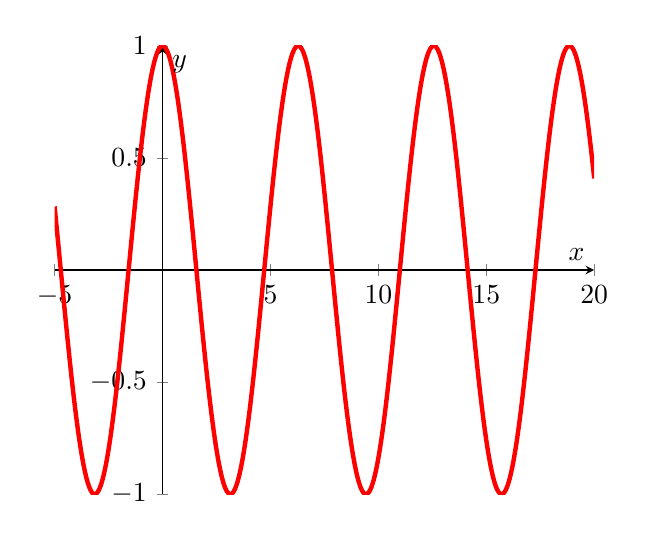
\begin{tikzpicture}
    \begin{axis}[
%    axis equal,
    samples=500,
    axis lines=middle,
    ylabel=$y$, 
    xlabel=$x$
    ]
    \addplot[domain=-5:20, black, ultra thick, color=red] {cos(deg(x))};
    \end{axis}
    \end{tikzpicture}
\end{center}
}

Now study the properties of $\cos(ax+b)$ in Geogebra:


\begin{center}
    \geogebra{zwrge8pa}{400}{300}
\end{center}



% Uncommented: sage doesn't work properly in the KU Leuven setup
%  -> see separate .tex file
\begin{comment}
\subsubsection{Do you know Sage?}

In Sage, you can relatively easily study the parametric equations of a circle:

\begin{sageCell}
    var('s t')
    x(t) = 3*cos(t)
    y(t) = 3*sin(t)
    c(t) = (x(t),y(t))
    circle=parametric_plot(c(t),(t,0,2*pi),color="black")
    circle
\end{sageCell}

\pdfOnly{In the online version you can experiment with this code. 

    See [some complicated url] or [a qrcode]
}

\begin{onlineOnly}

    Modify the code and press Evaluate!

    Nice, as they say ...

\begin{sageOutput}
    var('s t')
    x(t) = 3*cos(t)
    y(t) = 3*sin(t)
    c(t) = (x(t),y(t))
    circle=parametric_plot(c(t),(t,0,2*pi),color="black")
    circle
\end{sageOutput}
\end{onlineOnly}
\end{comment}

\xmsection{Styling}
	The online version can be styled by adding css files:
	\begin{itemize}
		\item \verb|global.css| in the root folder of the repository: all activities in the repository use this styling
		\item \verb|xoursefilename.css| in the folder of the xoursefilename.tex file: all activities in the xourse use this styling
		\item \verb|activityfilename.css| in the folder of the activityfilename.tex file: styling specific to one activity.
	\end{itemize}
	The \verb|ximeraShowcase.css| file in this case specifies that the questions have a purple bar not only on the left but also on the right side.


\end{document}